%!TEX root = ../dokumentation.tex

\chapter{Implementierung}

\section{BaklavaJS}

Eine der Anforderungen war es, das Modell visuell bearbeiten zu können. Dafür war es notwendig, einen Graph-Editor zu entwickeln. Ein solcher Editor erlaubt es, Knoten hinzuzufügen bzw. zu entfernen und sie miteinander zu verbinden.

Ein Knoten ist dabei wie eine mathematische Funktion: Er führt einen Algorithmus auf die Eingangsdaten aus und gibt die erzeugten Ausgangsdaten aus.

Visuell wird ein Knoten in BaklavaJS folgendermaßen dargestellt:

\begin{figure}[H]
    \centering
    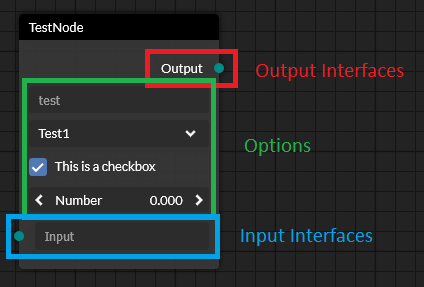
\includegraphics[width=.5\textwidth]{node_parts.png}
    \caption{Aufbau eines Knotens in BaklavaJS}
    \label{fig:nodeparts}
\end{figure}

Jeder Knoten besteht aus drei Teilen:
\begin{itemize}
    \item \textbf{Input Interfaces}: Die Eingangsschnittstellen eines Knotens werden benutzt, um Daten von anderen Knoten an diesen Knoten zu transferieren. Ist kein anderer Knoten verbunden, kann der Wert mittels eines Steuerelements auch direkt am Knoten eingestellt werden.
    \item \textbf{Options}: Hier können Werte eingestellt werden, die der Knoten für die Berechnung braucht, die aber beispielsweise zu komplex sind, um als Daten von anderen Knoten über Eingangsschnittstellen zu kommen.
    \item \textbf{Output Interfaces}: Die Ausgangsschnittstellen stellen das Ergebnis bereit, damit es von anderen Knoten benutzt werden kann.
\end{itemize}

\subsection{Ausführungsreihenfolge des Graphen}

\begin{figure}[H]
    \centering
    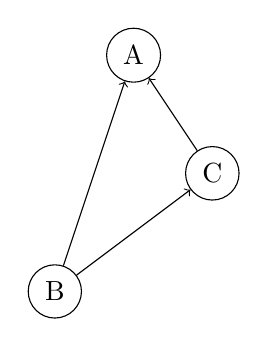
\begin{tikzpicture}
        \node[shape=circle,draw=black] (A) at (0,0) {A};
        \node[shape=circle,draw=black] (B) at (-1,-3) {B};
        \node[shape=circle,draw=black] (C) at (1,-1.5) {C};
        \path[->](B) edge node[left] {} (A);
        \path[->](B) edge node[left] {} (C);
        \path[->](C) edge node[left] {} (A);
    \end{tikzpicture}
    \caption{Beispielgraph}
    \label{fig:nodeExecutionOrder1}
\end{figure}

In Abbildung \ref{fig:nodeExecutionOrder1} ist ein Beispielgraph mit Knoten und Kanten zu sehen. Die Ausführungsreihenfolge der Knoten muss folgende Bedingungen erfüllen:
\begin{itemize}
    \item Jeder Knoten wird genau einmal ausgeführt
    \item Ein Knoten kann erst ausgeführt werden, wenn alle Knoten, die Kanten zu ihm haben, ausgeführt wurden
\end{itemize}

Um diese Anforderungen zu erfüllen, darf der Graph keine Zyklen enthalten. Mit folgendem Algorithmus kann die Ausführungsreihenfolge bestimmt werden:
\begin{enumerate}
    \item Adjazenzliste erstellen
    \item Baum aufbauen mit Zykluserkennung
    \item Breitensuche um die Ausführungsreihenfolge zu bestimmen 
\end{enumerate}

\begin{algorithm}[H]
    \caption{Baum aufbauen mit Zykluserkennung}
    \begin{algorithmic}[1]
        \Function{findDescendants}{treeNode, ancestors, adjacency}
            \ForAll{$c$ in $treeNode.children$}
                \If{$c$ in $ancestors$}
                    \State Cycle detected
                \EndIf
                \State $ancestors.push(c)$
                \State $c.children = findChildren(c)$
                \State \Call{findDescendants}{c, ancestors, adjacency}
                \State $ancestors.pop()$
            \EndFor
        \EndFunction
    \end{algorithmic}
\end{algorithm}

\begin{algorithm}[H]
    \caption{Breitensuche um die Ausführungsreihenfolge zu bestimmen}
    \begin{algorithmic}[1]
        \State $queue \gets \textbf{new} \ Queue()$
        \State $stack \gets \textbf{new} \ Stack()$
        \State $queue.push(root)$
        \While{\textbf{not} $queue.isEmpty()$}
            \State $current \gets queue.dequeue()$
            \ForAll{$c$ in $current.children$}
                \State $stack.push(c)$
                \State $queue.enqueue(c)$
            \EndFor
        \EndWhile
        \State $calculationOrder \gets \textbf{new} \ List()$
        \While{\textbf{not} $stack.isEmpty()$}
            \State $current \gets stack.pop()$
            \If{\textbf{not} $calculationOrder.contains(current)$}
                \State $calculationOrder.append(current)$
            \EndIf
        \EndWhile
    \end{algorithmic}
\end{algorithm}

Am Beispiel des Graphen in Abbildung \ref{fig:nodeExecutionOrder1} sieht der Algorithmus folgendermaßen aus:

\todo

\subsection{Grafische Umsetzung}

\subsubsection{VueJS}
VueJS ist ein JavaScript Framework zum Erstellen von Browser-Frontends. Ein wichtiges Konzept in Vue sind \textit{Komponenten}. Komponenten sind kleine, eigenständige und wiederverwendbare UI-Elemente. \url{https://vuejs.org/v2/guide/#Composing-with-Components}

In Anlehnung an das MVVM-Pattern (\url{https://vuejs.org/v2/guide/instance.html}) ist Vue \textit{reaktiv} gestaltet und bietet Datenbindung. Reaktiv bedeutet, dass Daten im sogenannten \textit{ViewModel} geändert werden können und diese Änderungen direkt in der \textit{View} angezeigt werden. \todo{Grafik zur Verdeutlichung}

Diese Art der Wiederverwendbarkeit ist essentiell, um die Knoten und Kanten zu zeichnen. Besonders hilfreich ist hierbei die \texttt{v-for}-Direktive. Sie erlaubt es, eine Liste von Komponenten zu rendern. Dabei werden Änderungen in der Liste über Datenbindung direkt in der UI übernommen. \todo{Mehr Erklärung}



\begin{itemize}
    \item Erklärung VueJS
    \item Wie werden die Kanten gezeichnet?
    \item Wie werden NodeOptions gezeichnet?
    \item Wie wird Zoom / Panning umgesetzt?
\end{itemize}

\subsection{Plugin-System und Event-System}

\subsection{BaklavaJS Pakete}
\begin{itemize}
    \item Core
    \item Engine
    \item Interface-Types
    \item Vue-Renderer
    \item Vue-Options
\end{itemize}

\section{Datengenerierung}

\begin{itemize}
    \item Worker / Multithreading
    \item Gefailter Ansatz mit Streamsaving
\end{itemize}

\section{Random Sampling / Custom Random}

\section{Build-System / Webpack}
\begin{itemize}
    \item Code-Splitting / Bundle-Optimization
\end{itemize}